\documentclass[a4paper,12pt]{article}
%\documentclass[14pt,a4paper,twoside]{report}
\usepackage[T2A]{fontenc}
\usepackage[utf8]{inputenc}			%включаем свою кодировку: koi8-r или utf8 в UNIX, cp1251 в Windows
\usepackage[english,russian]{babel}		%используем русский и английский языки с переносами
\usepackage{amssymb,amsfonts,amsmath,mathtext,cite,enumerate,float} %подключаем нужные пакеты расширений
\usepackage[dvips]{graphicx}			%хотим вставлять в диплом рисунки?
%\usepackage{soul}
\usepackage[14pt]{extsizes}
\usepackage{longtable} 
\usepackage{graphicx}
\usepackage{indentfirst}
\usepackage{enumerate}

\graphicspath{images/}			%путь к рисункам
\bibliographystyle{unsrt}			% for bibtex

%\linespread{1.5}

\usepackage[format=plain,labelformat=simple,labelsep=endash,figurename=\CYRR\cyri\cyrs\cyru\cyrn\cyro\cyrk]{caption}
%\captionsetup{figurewithin=section}		% картинки нумеруются относительно секций
%\numberwithin{equation}{section}		% нумерация формул внутри раздела
\numberwithin{table}{section}

\makeatletter
\renewcommand{\@biblabel}[1]{#1.} 		% Заменяем библиографию с квадратных скобок на точку:
\makeatother

\RequirePackage{lscape}

\usepackage{geometry} 				% Меняем поля страницы
\geometry{left=2cm}				% левое поле
\geometry{right=1cm}				% правое поле
\geometry{top=2cm}				% верхнее поле
\geometry{bottom=2cm}				% нижнее поле

\renewcommand{\theenumi}{\arabic{enumi}}	% Меняем везде перечисления на цифра.цифра
\renewcommand{\labelenumi}{\arabic{enumi}}	% Меняем везде перечисления на цифра.цифра
\renewcommand{\theenumii}{\arabic{enumii}}	% Меняем везде перечисления на цифра.цифра
\renewcommand{\labelenumii}{\arabic{enumi}.\arabic{enumii}.}% Меняем везде перечисления на цифра.цифра
\renewcommand{\theenumiii}{\arabic{enumiii}}	% Меняем везде перечисления на цифра.цифра
\renewcommand{\labelenumiii}{\arabic{enumi}.\arabic{enumii}.\arabic{enumiii}.}% Меняем везде перечисления на цифра.цифра

\begin{document}

\title{Создание лабораторного стенда для приема сигналов спутниковых систем навигации.}
\author{Мельников А.О\\ melnikov.aleksey@rf-lab.org\\ МГУПИ \and Никифоров А.А.\\nikiforov.alex@rf-lab.org\\ МГУПИ}

\maketitle

\begin{abstract}
Данная статья посвещена современным методикам получения и обработки сигнала спутниковых радионавигационных систем (СНРС) в
приложении к учебному процессу в ВУЗ. Рассмотрены возможные решения, а так же проанализированы достоинства и недостатки
решений. В заключительной части представлена типовая схема программного приемника, кратко рассмотрена структура
СНРС сигнала системы Navstar GPS и показан пример работы одного из возможных алгоритмов по поиску сигнала заданного спутника - 
схема параллельного коррелятора. 
\end{abstract}

\section{Введение}
Изучение современных беспроводных систем передачи данных предполагает проведение большого количества
практических занятий с использованием лабораторного оборудования.
Организация таких занятий требует значительных финансовых затрат на приобретение оборудования и поддержку его работоспособности.
В этой статье мы хотели бы рассмотреть основные подходы к организации стенда для анализа сигналов систем спутникового позиционирования (СНРС).

На данный момент на рынке СНРС решений представлено 3 системы: Navstar GPS, Galileo, ГЛОНАСС. Система GPS использует методику
расширения спектра с кодированием CDMA \cite{gpsuserequipment}, в то время как Galileo и ГЛОНАСС используют частотное разделение \cite{galileo}
 
Будет рассмотрено три основных подхода к организации подобной лаборатории от самого дорогого, при котором используется профессиональное измерительное
оборудование с для поиска и анализа СНРС сигнала, до самого дешевого, но вместе с тем очень захватывающего, когда все придется делать своими руками.
В первом случае понадобятся: антенна GPS/GLONASS, демодулятор (downconvertor),
векторный анализатор сигналов и соединительные кабели. Основная стоимость в этом случае приходится на векторный анализатор сигналов (VSA).
Этот прибор позволяет осуществлять захват измеряемого сигнала, с возможностью его последующего анализа в оцифрованном виде.

\section{Варианты????}
В сценарии записи сигнала может использоваться комплекс от компании NI с VSA, такой как NI PXI-5661 рисунок \ref{pic:ni5661}
(картинка взята с сайта \cite{ni5661}.
Используя данную сборку, можно получить необходимый кусок "сырого" сигнала для последующей обработки.
Для каждого типа беспроводной связи требования к ширине полосы пропускания, центральной частоте и требуемое усиление разные. В
случае GPS, основным является захват 2.046МГц полосы пропускания с центральной частотой 1.57542ГГц.
Так как мощность реальнго GPS сигнала очень низка, для записи так же необходим малошумящий усилитель, такой как PXI-5690.
Также компания поставляет набор программного обеспечения для анализа  GPS сигналов - NI GPS Toolkit для LabVIEW.
Обзор данного решения представлен в \cite{ni5661, ni-vsa}.
К несомненным достоинствам данного решения относятся готовый набор качественного программного и аппаратного обеспечения.
Данное решение используется крупными компаниями для разработки и тестирования GPS приемников.
 
\begin{figure}[h]
\begin{center}
    \scalebox{0.8}{\includegraphics[width=1\linewidth]{./images/ni5661.eps}}
\end{center}
\caption{Комплекс от компании NI}
\label{pic:ni5661}
\end{figure}

Второй подход основан на использовании стартовых или отладочных наборов для микросхем приема сигналов GNSS.
Стоимость такого набора может варьироваться от сотен долларов до нескольких тысяч.
В набор обычно входят: специализированное аппаратное обеспечение (АО), иногда включается программное обеспечение (ПО).
Качество и функциональный набор ПО может варьироваться.
Данные отладочные наборы предназначены для отладки программного и аппаратного обеспечения, использующего набор
микросхем, расположенных на отладочной плате.
В качестве примера можно привести отладочную плату от компании Maxim Semiconductor на базе микросхемы GPS приемника MAX2769 \cite{max-evkit}.
Стоимость платы, при покупке на сайте производителя, составляет 550\$.
Программное обеспечение для данной платы позволяет перепрограммировать микросхему в разные режимы работы.
Никакого программного обеспечения обработки сигнала на сайте не обнаружено.

В виду высокого интереса к данной теме, некоторые университетские команды разрабатывают собственное ПО и АО 
для захвата и обработки GNSS сигналов.
Как пример можно привести проект softGPS.
В рамках этого проекта разработано ПО демодуляции спутникового сигнала, работающее с различными адапторами сбора данных
(АСД - front-end) устройствами.
Одним из возможных вариантов для работы может являться высокочастотный (RF) АСД разработанный Денисом Акосом (Dennis Akos) \cite{akos-frontend}.
Стоимость данного устройства составляет 450\$.
Так же заслуживает отдельного внимания методология программного приемника (ПП - software reciever).
В рамках данного подхода вся обработка сигнала ведется на программном уровне (идеальный программный приемник обрабатывает также 
высокочастотный тракт).
Преимуществом данного подхода является низкая стоимость разработки приемника.
Обрабатывая данные на специализированных математических пакетах (Matlab, Octave), пользователь может реализовать достаточно сложные алгоритмы в примлемые
временные рамки и без финансовых вложений в разработку аппаратных решений. Это позволяет заниматься обработкой сигналов даже любителям
рисунок \ref{pic:sdr}.

\begin{figure}[h]
\begin{center}
    %\scalebox{1}{\includegraphics[width=1\linewidth]{./images/board.eps}}
    %\includegraphics[width=1\linewidth]{./images/board_main.eps}
\end{center}
\caption{Схема программного приемника}
\label{pic:sdr}
\end{figure}

Третий подход предполагает самостоятельное изготовление приемно-измерительного оборудования.
Такой подход, безусловно, является очень гибким и самым дешевым из рассматриваемых, но требует дополнительных навыков.
Так же преемуществом данного подхода является доступ к полной спецификации аппаратного обеспечения и возможнсть
разработки своего варианта программного обеспечения.
Это, безусловно, является достаточно трудоемкой задачей, но в процессе решения реализуется непосредственный
смысл разработки - создание стенда для проведения лабораторных работ.

Рассмотренные решения позволяют оценить плюсы и минусы каждого.
К недостаткам VSA-устройств можно отнести высокую стоимость, но вместе с тем они обладают огромным функционалом.
При использовании отладочных наборов появляется проблема в том, что они ориентированы на прототипирование аппаратной
части и, зачастую, обладают очень скромным сопроводительным ПО.
Достаточно интересным решением может быть проект softGPS.
Цена данного решения, относительно VSA-устройств, гораздо более привлекательна для конечного пользователя
(в отличае от крупных компаний), но все же достаточно высока.

Рассмотрев варианты, мы приняли решение разработать свой АСД-модуль и ПО.

% ####################################################################3
\section{Cтруктура СНРС сигнала системы Navstar}

Рассмотрим структуру сигнала в СНРС GPS. В GPS применяется фазововая схемы модуляции при кодировании информационных битов.
Фазовава манипуляция (phase shifting key - PSK).  Она была разработана  в начале развития программы исследования дальнего космоса;
сейчас схема PSK широко используется в коммерческих и военных системах связи. Фазоманипулированный сигнал имеет следующий вид \cite{sklyar}:

\begin{eqnarray}
s_i=\sqrt{\frac{2E}{T}}\cos{[{{\omega}_0}t + \phi_i(t)]}, \nonumber \\
	0\leq{t}\leq{T}, i = 1, ..., M.
\label{eq:bpsk}
\end{eqnarray}
В данном случае фазовый член ${\phi_t(t)}$ может принимать ${M}$ дискретных значений. Для случая модуляции в GPS системе ${M=2}$.
\begin{eqnarray}
	\phi_i(t)=\frac{2\pi{i}}{M}=\pi{i} \nonumber \\
	i = \{1,2\}.
\label{eq:bpsk_phi}
\end{eqnarray}
На рисунке \ref{pic:bpsk} представлена схема двочной модуляции - показан переход битов 101. В формуле \ref{eq:bpsk}, ${E}$ - это энергия
сигнала, ${T}$ - время передачи символа, ${0\leq{t}\leq{T}}$. Работа схемы заключается в смещении фазы модулируемого сигнала
${s_i(t)}$ на одно из двух значений нуль(${2\pi}$) или ${\pi}$. На рисунке \ref{pic:bpsk} явно видно характерное изменение фазы при 
переходе между символами.

\begin{figure}[h]
\begin{center}
	\scalebox{0.8}{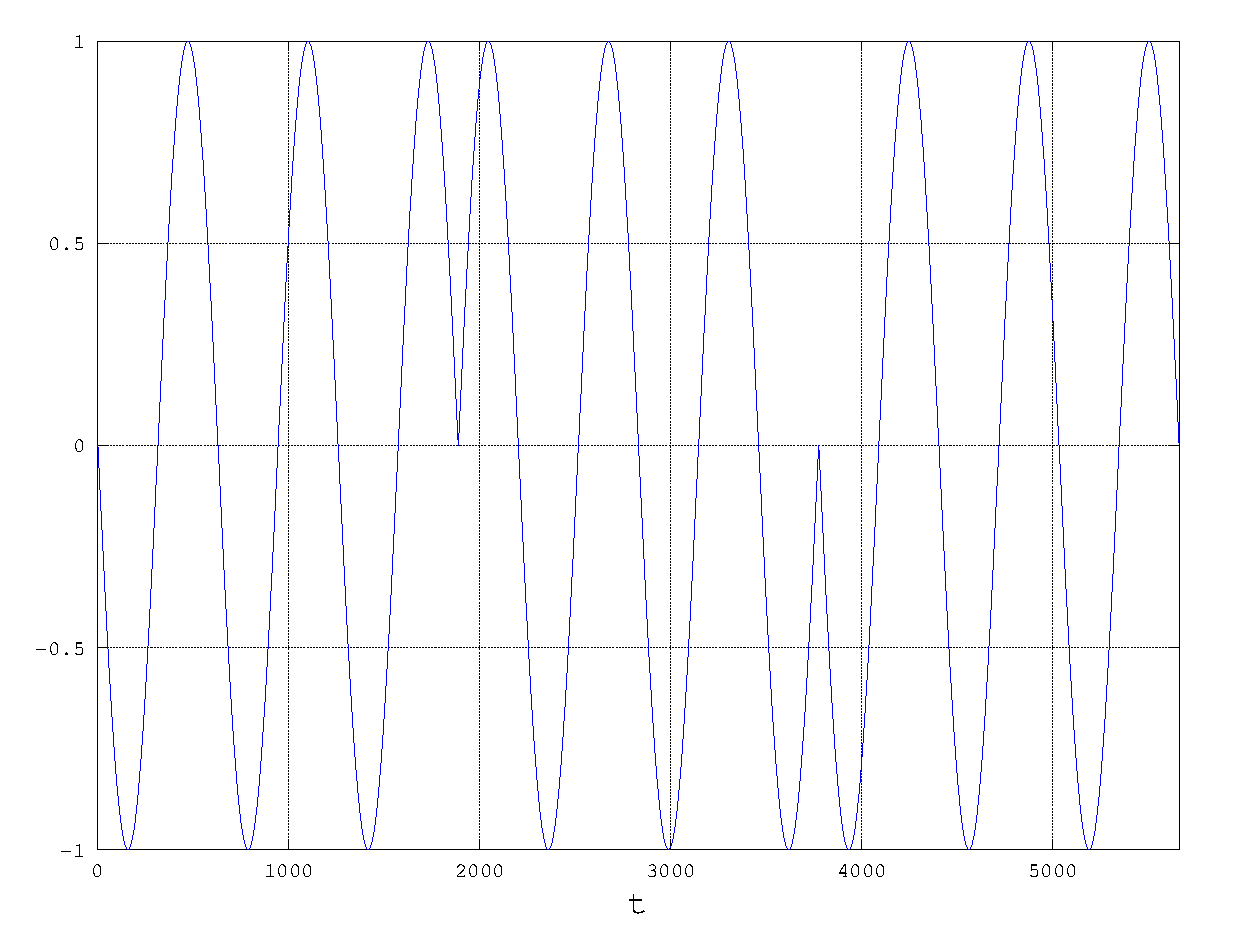
\includegraphics[width=1\linewidth]{./images/bpsk.eps}}
\end{center}
\caption{Схема модуляции BPSK}
\label{pic:bpsk}
\end{figure}

В системах GPS применяется кодовое разделение каналов. В качестве кода применяется семейство кодов Голда \cite{gold-ieee}.
Код Голда представляет собой псевдослучайную последовательность (ПСП). Спектр ПСП близок к шуму, а значит его
спектральная плотность мощность (СПМ) близка к равномерной в диапазоне ${[-2\pi{f_{clk}^{C}};2\pi{f_{clk}^{C}}]}$, где
${f_{clk}^{C}}$ - частота генерации кода. В результате мощность первоначального сигнала окажется "размыта" в диапазоне 
${[-2\pi{f_{clk}^{C}};2\pi{f_{clk}^{C}}]}$, который в ${\frac{f_{clk}^{C}}{f_{clk}^{D}}}$, где ${f_{clk}^{D}}$ - частота
исходных данных. Стоит отметить несколько фактов, почему именно коды Голда были выбраны в качестве ПСП в GPS системах. 
В \cite{gold-ieee} приводится доказательство, того, что определенным образом сгенерированные ПСП, будут обладать заданными
корреляционными свойствами. Генераторы ПСП (в GPS их используется 2) подробно рассмотрены в \cite{tsui, akos-book}. 
Автокорреляционный пик ПСП, очевидно, равен:
\begin{eqnarray}
	R = 2^n -1 = 1023 
\label{eq:ca_peak}
\end{eqnarray}
Так в генераторах ПСП GPS систем 10 бит. Но гораздо более важным является значение корреляции кода со своей сдвинутой во
времени копией. Для семейства кодов Голда это значение определяется соотношением:
\begin{eqnarray}
	\left|{R}\right| \leq 2^{(n+2)/2} + 1 = 65
\label{eq:ca_peak}
\end{eqnarray}

\begin{figure}[h]
\begin{center}
	\scalebox{0.8}{\includegraphics[width=1\linewidth]{./images/ca_xcorr.eps}}
\end{center}
\caption{Автокорреляция кода Голда}
\label{pic:gold}
\end{figure}
На рисунке \ref{pic:gold} представлен график корреляции кода Голда. Максимальное значение на графике равно 1023, коррреляция 
со сдвинутой во времени копией не превышает 65, полученные значения соответствуют данным из \cite{gold-ieee}.

% ####################################################################3
\section{Наш собственный АСД}
Выбрав для реализации малобюджетную GPS микросхему MAX2769 компании Maxim Semiconductor, мы разработали плату под управлением ПЛИС Xilinx Spartan 2E
(рисунок \ref{pic:our-board}).
Данная плата оснащена микросхемой статической памяти 256Кб.
Что позволяет сохранить чуть более 32 мс оцифрованных данных при скорости оцифровки 16.368 Мгц.
Данного объема данных хватает для реализации лабораторной работы по обнаружению спутников.

\begin{figure}[h]
\begin{center}
    \scalebox{1}{\includegraphics[width=1\linewidth]{./images/board.eps}}
    %\includegraphics[width=1\linewidth]{./images/board_main.eps}
\end{center}
\caption{Структурная схема платы}
\label{pic:our-board}
\end{figure}

В одной из простых реализаций коррелятора необходимо обрабатывать 1 мс данных.
Для более точной оценки частоты требуется 5 мс данных (алгоритм основанный на разности фаз).
Таким образом, такой конфигурации вполне достаточно для реализации поставленной задачи с минимальными
финансовыми затратами на программное и аппаратное обеспечение.
ПО управления платой, а так же VHDL код управления микросхемами на плате были реализованы нами.
Референсное ПО обнаружение спутников так же было разработано нами на Matlab/Octave с использованием подходов рассмотренных в \cite{tsui}.

Оборудование захвата представляет собой специализированный приемник сигнала GPS, позволяющий осуществить запись фрагмента сигнала от спутников.
Записанный сигнал поступает на сервер захвата и далее записывается в виде файла на публичный сервер FTP.
В текущей конфигурации \cite{gpsproject} периодически сохраняется текстовый файл flush содержащий отрезок сигнала и изображение waas\_sats с
положением спутников. Оборудование захвата содержит высокочастотный тракт, микросхему программируемой логики, память размером 256 Кбайт
для временного хранения сигнала и интерфейс RS-232 для передачи измеренного сигнала из памяти в основной сервер системы захвата.

Сигнал спутника на частоте 1575.42МГц поступает на вход малошумящего усилителя (МШУ) и далее через ПАВ фильтр на модуль смесителя.
После смесителя выделяются две квадратурные компоненты на промежуточной частоте 4.092 МГц.
Эти сигналы поступают на двухбитовые аналого-цифровые преобразователи с частотой дискретизации 16.368 МГц (рисунок \ref{pic:our-board}).
Микропрограммное обеспечение осуществляет заполнение памяти захваченным сигналом и дальнейшую передачу этой информации
по порту RS-232 на основной сервер. Сервер осуществляет пересылку сигнала на публичный сервер ftp в виде текстового
или бинарного файла.

% ####################################################################3
\section{Алгоритм параллельного коррелятора}

К данному моменту нами рассмотрены основные составляющие системы GPS: приемное оборудование, система кодирования информации,
а так же система мультиплексирования данных от разных спутников, работающих на одной частоте. В заключительной части хотелось
бы рассмотреть один из алгоритмов захвата спутникового сигнала - определение наличия сигнала спутника 
в полученных данных. Мы воспользуемся разработанной нами АСД для Navstar GPS, а так же
свободным математическим пакетом Octave (бесплатный аналог пакета Matlab).

Определение наличия сигнала спутника с номером N в данных производится с помощью кросскорреляции между локально-сгенерированным
сигналом и сигналом полученным с АСД. На вход коррелятора поступает входной
сигнал, коррелятор генерирует несущую и ПСП. Далее коррелятор производит кросскорреляцию входного сигнала и сгенерированного. 
На выходе коррелятора стоит пороговый детектор, определяющий есть ли сигнал от спутника N в данных. Поиск производится в 
двух измерениях: по времени и по частоте. Остановимся на этом более подробно. За счет движения спутника (а так же, возможно,
и приемника) частота, на которой работает спутник, искажается за счет эффекта Допплера. Для стационарных и медленно движущихся
приемников данное искажение находится в  пределах ${\pm{5 \mbox{кГц}}}$ \cite{tsui}. Так же мы не знаем смещение кода C/A
внутри сигнала. В результате получается, как указано выше, поиск в двух измерениях: поиск по частоте смещения Допплера и
поиск по фазе C/A кода. Для решения данной задачи, нам необходимо посчитать корреляцию (формула \ref{eq:corr}) с одинадцатью
последовательностями, каждую последовательность прокоррелировать 1023 раза с входящим сигналом.
В итоге мы получим вектор значений корреляции.

\begin{eqnarray}
	z(n) = \sum_{m=0}^{N-1}{x(m)h(n+m)}
\label{eq:corr}
\end{eqnarray}

Как показано в \cite{oppenheim, tsui}, процедуру корреляции можно немного оптимизировать за счет осуществления корреляции через
БПФ. Используя известное соотношение, что свертка во временной области равна умножению в частотной, можно получить корреляцию по
всем 1023 смещениям умножив последовательности в частотной области. Данный алгоритм называется параллельный коррелятор.
В формуле \ref{eq:par_corr} представлена цепочка операций.

\begin{eqnarray}
	z(n)	= \mathcal{F}^{-1}(\left|{Z(k)}\right|)
		= \mathcal{F}^{-1}(\left|{H^*(k)X(k)}\right|)
		= \mathcal{F}^{-1}(\left|{H(k)X^*(k)}\right|)
\label{eq:par_corr}
\end{eqnarray}
Где ${H^*(k)}$ - комплексно-сопряженное число, а ${\mathcal{F}^{-1}}$ - обратное преобразование Фурье. Схема параллельного коррелятора
представлена на рисунке \ref{pic:par_corr}.
\begin{figure}[h]
\begin{center}
	\scalebox{0.8}{\includegraphics[width=1\linewidth]{./images/fft.eps}}
\end{center}
\caption{Схема параллельного коррелятора}
\label{pic:par_corr}
\end{figure}
Весь парралелизм идеи состоит в том, что корреляцию локального и полученного сигнала по всем смещениям C/A кода
можно провести за 4 операции: преобразование фурье входного и локального сигнала, умножение и обратное преобразование
фурье. В результате получается вектор с корреляциями по всем возможным смещениям C/A кода.

\begin{figure}[h]
\begin{center}
	\scalebox{0.8}{\includegraphics[width=1\linewidth]{./images/corr_bar.eps}}
\end{center}
\caption{Корреляция всей группировки спутников Navstar GPS}
\label{pic:corr_bar}
\end{figure}

Рассмотрев все теоретические аспкеты системы Navstart GPS, мы представим результаты работы алгоритма "параллельного коррелятора".
Теоритические аспекты данного алгоритма подробно разобраны в \cite{tsui, akos-book}. Многие статьи, которые нам встречались,
производят тестирование алгоритмов захвата и сопровождения сигнала на тестовом сигнале. Мы же работаем с реальным сигналом,
полученным с помощью нашего АСД. Для примера возьмем файл и запустим коррелятор. Результат работы коррелятора для нашего
дампа приведен на рисунке \ref{pic:corr_bar}. Очевидно видны высокие значения корреляции для спутников 30, 31, 32.
%Исследуем более подробно данные спутники.
\begin{figure}[h]
\begin{center}
	\scalebox{0.8}{\includegraphics[width=1\linewidth]{./images/corr_30_4092.eps}}
\end{center}
\caption{Корреляция спутника PRN=30}
\label{pic:corr_30}
\end{figure}
Для спутника с PRN=30, значение корреляции равно 25027615.13340 при смещении C/A кода 4777 чипа на частоте 4094000 Гц.
%
%\begin{figure}[h]
%\begin{center}
%	\scalebox{0.8}{\includegraphics[width=1\linewidth]{./images/corr_31_4092.eps}}
%\end{center}
%\caption{Корреляция 31 спутника}
%\label{pic:corr_31}
%\end{figure}
%Спутника с PRN=31, представлен на рисунке \ref{pic:corr_32} имеет самое высокое значение корреляции
%54253119.99998 при смещении C/A кода 13862 чипа на частоте 4092000 Гц.
%
%\begin{figure}[h]
%\begin{center}
%	\scalebox{0.8}{\includegraphics[width=1\linewidth]{./images/corr_32_4092.eps}}
%\end{center}
%\caption{Корреляция 32 спутника}
%\label{pic:corr_32}
%\end{figure}
%Спутник (рисунок \ref{pic:corr_32}) с PRN=32 имеет значение корреляции 47114911.99999 при
%смещении C/A кода 08157 чипа на частоте 4092000 Гц.

\begin{figure}[h]
\begin{center}
	\scalebox{0.8}{\includegraphics[width=1\linewidth]{./images/corr_05_4092.eps}}
\end{center}
\caption{Корреляция 5 спутника}
\label{pic:corr_5}
\end{figure}
Из рисунка \ref{pic:corr_5} видно, что спутник c PRN=5 явных корреляционных пиков не имеет.

Стоит отметить, что точность коррелирования на этапе захвата зависит от длинны данных, подвергающихся преобразованию фурье.
Мы использовали 1 мс данных и наша точность не превышает 500 Гц. Так же хочется отметить, что максимальная корреляция на 
первом этапе совсем не означает лучший уровень сигнала. Вполне возможно, что у любого другого спутника смещение частоты
находится около 500 Гц, в этом случае корреляционный пик будет совсем слабо выражен, так как частота входного сигнала
сильно отличается от частоты внутреннего генератора. Существует метод повышения точности опеределения частоты
входного сигнала основанный на вычислении фазы сигнала. Данный подход описан в \cite{tsui}, но как в описании, так и в
реализации алгоритма в данном источнике допущены существенные опечатки. Так же данные опечатки нам встретились 
в нескольких зарубежных статьях.

В данной статье мы рассмотрели типовые решения получения сигнала для системы Navstar GPS. Варианты систем
как от крупной компании National Instruments, так и разработки частных лиц - применик Денниса Акоса. 
Так как наши цели и бюджеты несколько отличались от характеристик и стоимости приведенных аналогов, мы разработали
свою плату получения сигнала Navstar GPS на частоте L1, работая в истинно университетском духе - разрабатывая все сами.
Далее в статье мы представили базовые понятия, необходимые для понимания специфики кодирования сигнала в  GPS и
представили один из алгоритмов захвата спутникового сигнала - параллельный коррелятор. Был представлен
результат работы параллельного коррелятора. Все разработанные коды являются открытыми и вы сами можете легко проверить
все результаты работы. Исходные коды доступны по адресу \cite{gpsproject}, а так же на вебсайте нашего проекта www.rf-lab.org.
Получить дамп, использованный в этой статье вы так же можете на вышеуказанном сайте.

\bibliography{../../bibtex_db}

\end{document}
